A 2D free field effective stress analysis is performed by s$^3$hark
and demonstrated here.  The results are verified against FLAC and
Plaxis.  The soil column being analyzed is 6 meters high sitting on a
rock.  The ground water table is at 2 meters below the soil surface.
In the column, there are a total of three soil layers. Each layer is
meshed by elements with a size of 0.25 meter in height.  Basic
properties of soil layers and the rock are shown
in \Cref{fig:s3harkSoilColumn} and \Cref{fig:s3hark5}.  The
first two layers are modeled by PM4Sand and the third layer is modeled
by elastic isotropic material.  (The implementation work of
PM4Sand \cite{boulanger2015pm4sand} is done in University of
Washington by Long Chen and Pedro Arduino.  Chaofeng Wang at UC,
Berkeley contributed to the code optimization for speed improvement. )
The rock layer will be simplified to a \cite{Lysmer:1969} dashpot,
which accounts for the finite rigidity of the underlying elastic
medium.  The parameters of the dashpot are calculated solely based on
rock layer's density and V$_{s30}$.


\begin{figure}[!htbp]
  \centering {
    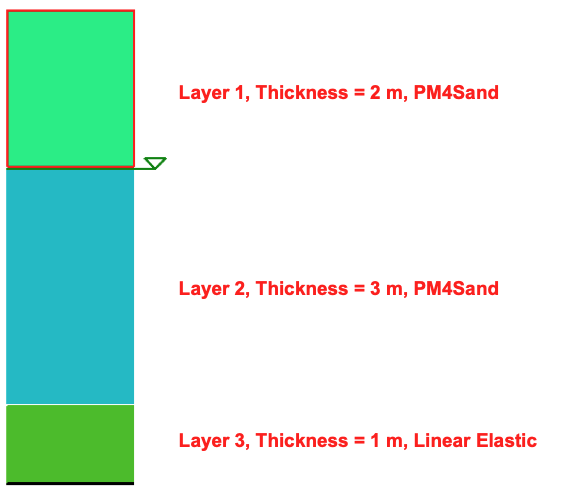
\includegraphics[width=0.5\textwidth]
    {ver_and_val/figures/s3harkSoilColumn.png} }
  \caption{Soil layers }
  \label{fig:s3harkSoilColumn}
\end{figure}


\begin{figure}[!htbp]
  \centering {
    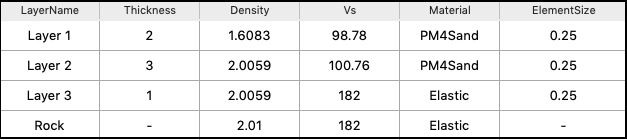
\includegraphics[width=0.5\textwidth]
    {ver_and_val/figures/s3hark5.png} }
  \caption{Soil layers }
  \label{fig:s3hark5}
\end{figure}


The detailed properties of the material in each soil layer are shown in \Cref{fig:s3hark6}.

\begin{figure}[!htbp]
  \centering 
  \subfloat[Layer 1]{
    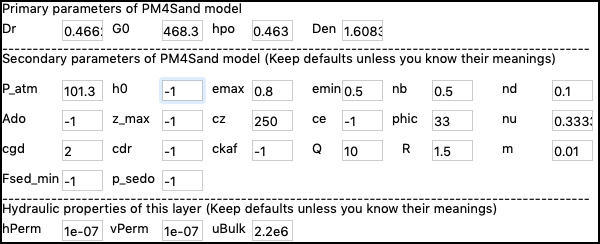
\includegraphics[width=0.4\textwidth]
    {ver_and_val/figures/layer1.png}}
  \subfloat[Layer 2]{
    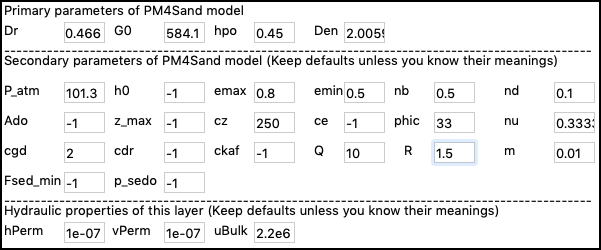
\includegraphics[width=0.39\textwidth]
    {ver_and_val/figures/layer2.png}}
    
    \subfloat[Layer 3]{
    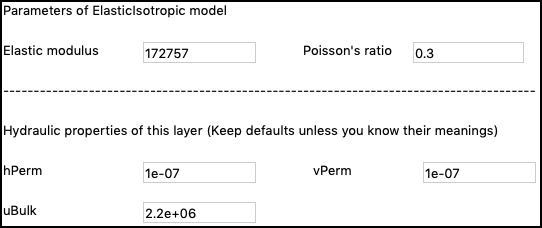
\includegraphics[width=0.4\textwidth]
    {ver_and_val/figures/layer3.png}}
  \caption{Detail soil properties and material model parameters}
  \label{fig:s3hark6}
\end{figure}

For the verification and validation purposes, s$^3$hark's results are compared with FLAC an PLAXIS, as shown in \Cref{fig:s3hark7}. 
All three programs generally produce very similar response with
different levels of differences shown in PHA, maximum shear strain, CSR, maximum pore pressure ratio. 
The differences come from multiple sources, such as numerical discretization methods, solvers, etc.
For example, FLAC tends to produce higher dilation pulses in liquefied layer. 
This is possibly due to a combination of different reasons, e.g.,
interpolation of data from integration points at different
locations, numerical methods for integration, formulations for
solid fluid coupling, etc.
(Chaofeng Wang at UC, Berkeley, Long Chen and Andrew Makdisi at University of Washington,  
Gregor Vilhar at PLAXIS, BV contributed to the verification of PM4Sand in s$^3$hark. )

\begin{figure}[!htbp]
  \centering {
    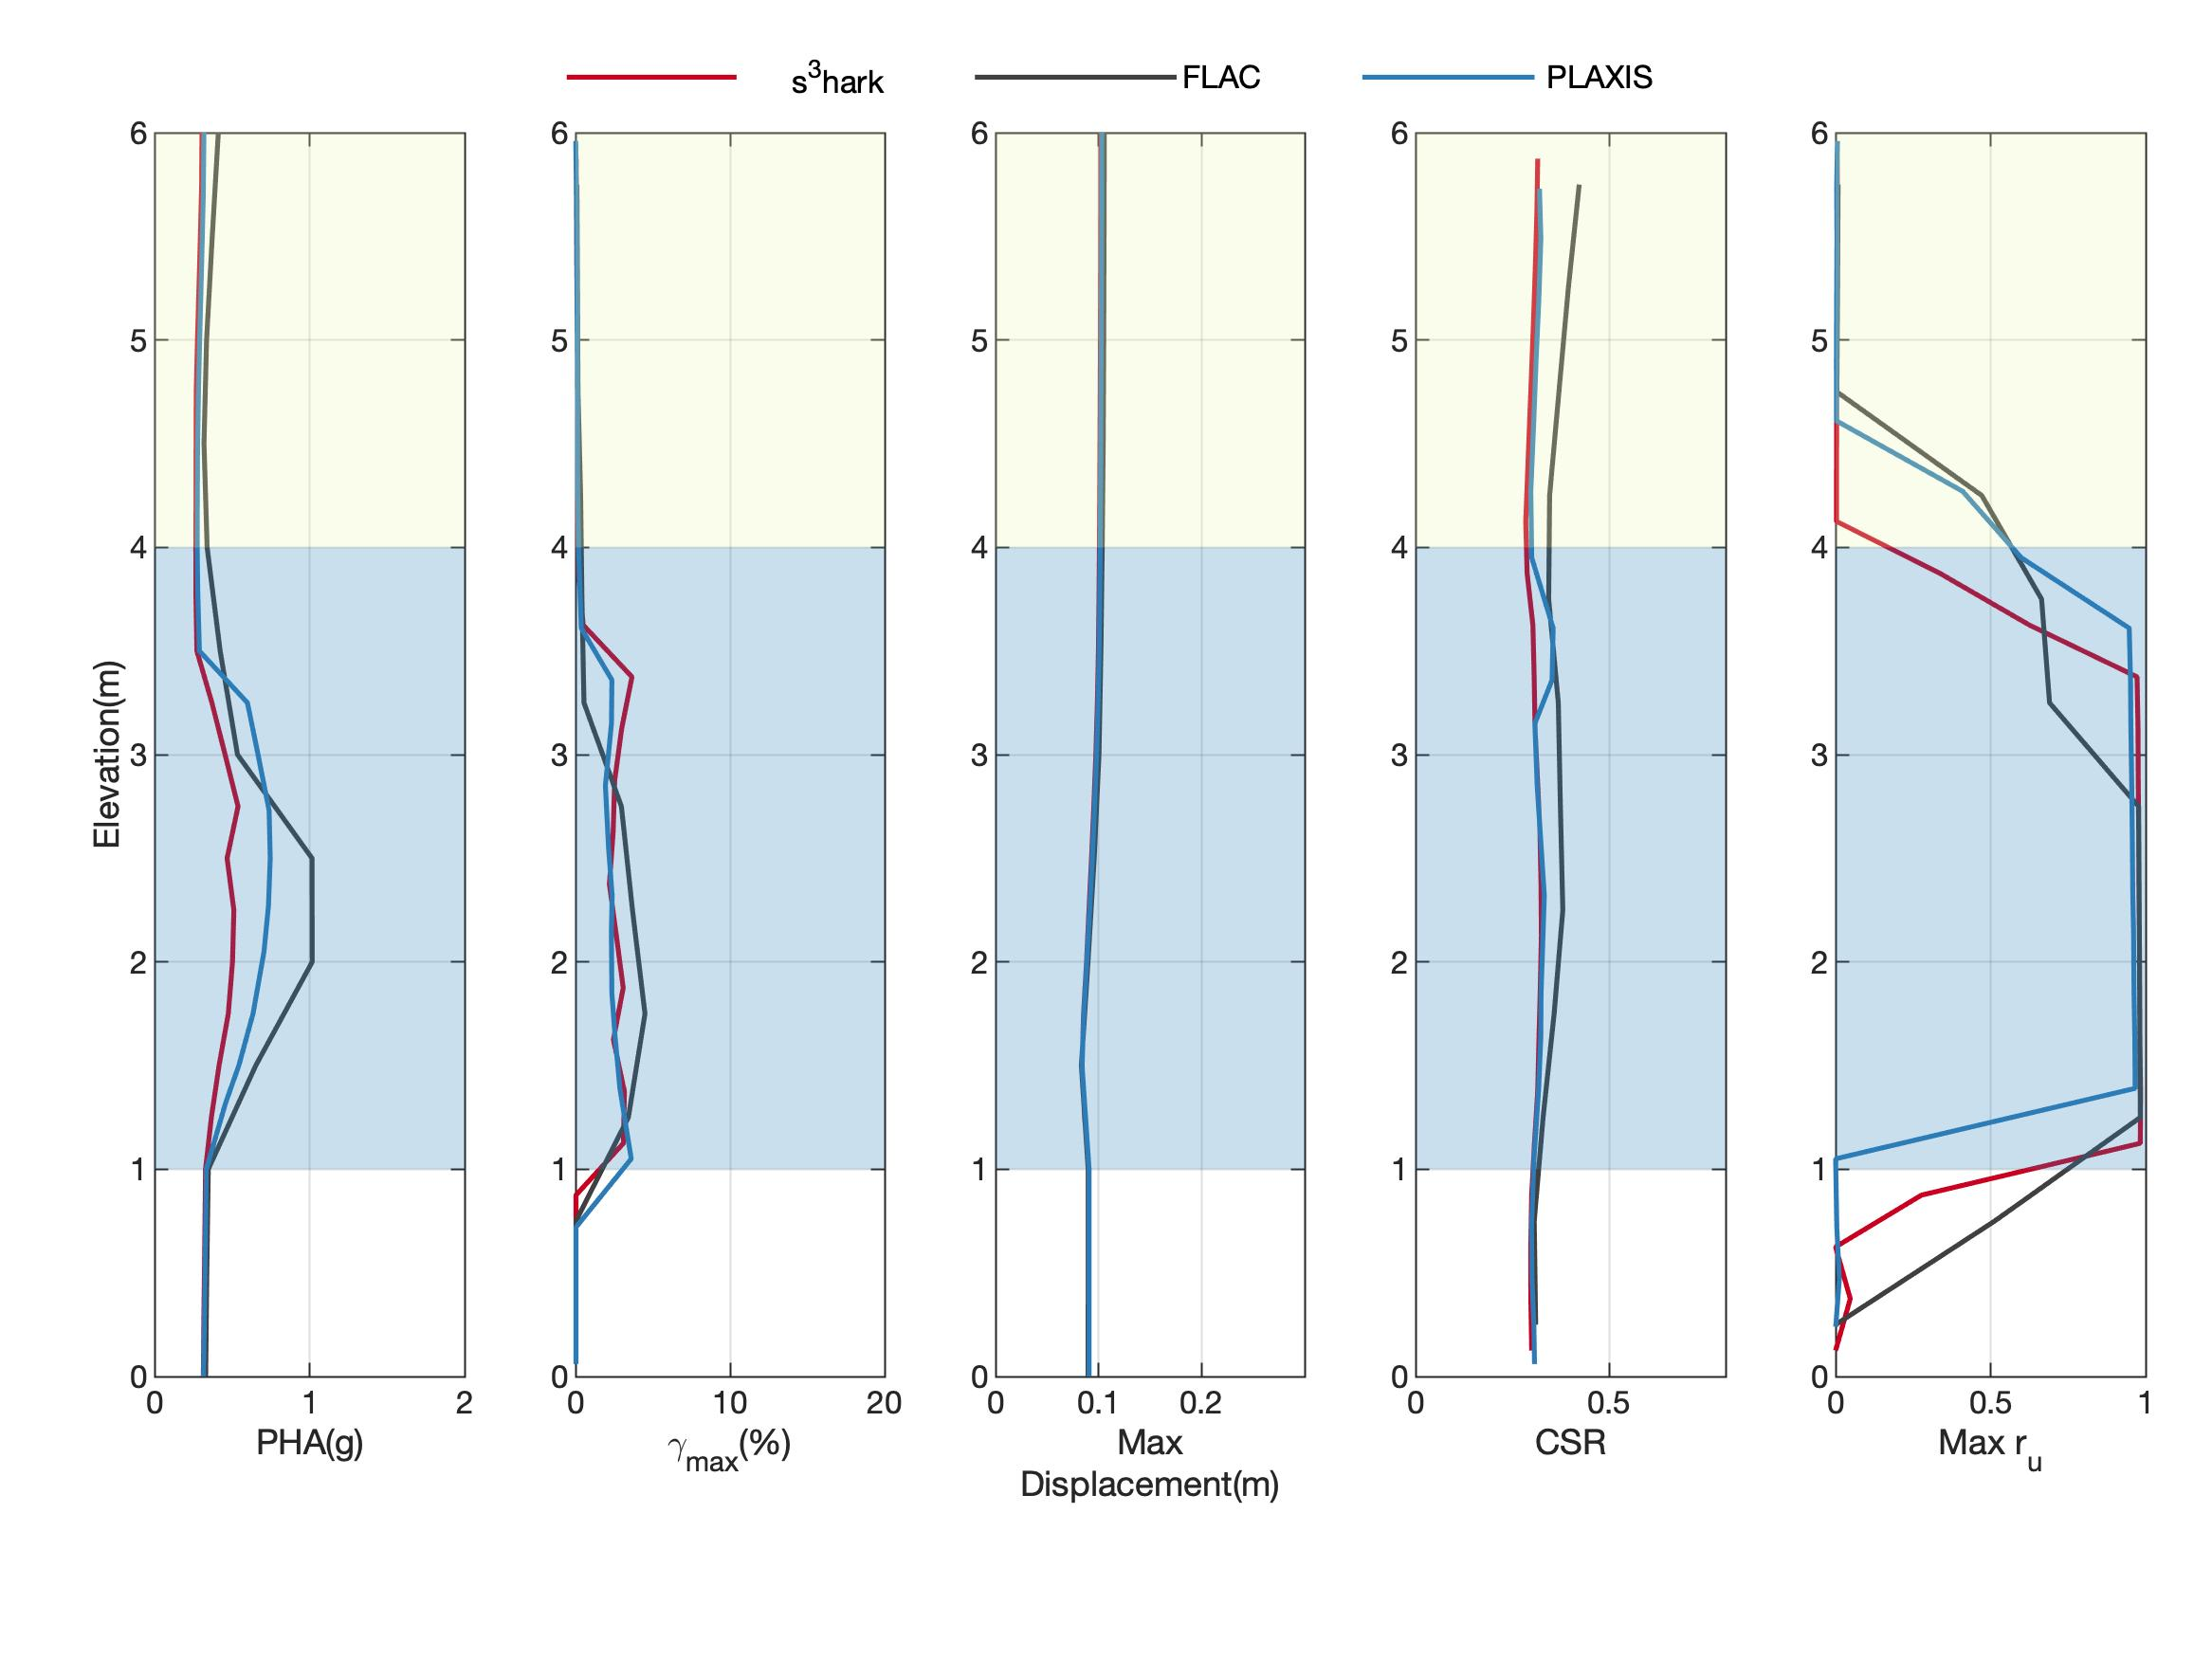
\includegraphics[width=0.7\textwidth]
    {ver_and_val/figures/N10T3_RSN766_ProfileCompare.jpg} }
  \caption{Soil layers }
  \label{fig:s3hark7}
\end{figure}
